\scanpage{5}
\mspage{4}
\uline{Lieu} sur une ficelle $(X,\{A,B\})$ ;
c'est une partie \inserted{fermée} $C\subset X$ telle que
l'on ait les propriétés : ou bien $C\in\{A,B\}$,
ou bien les propriétés suivantes sont satisfaites.

\margin{\uline{NB} \inserted{Pour} une ficelle réduite $(X',\{a,b\})$,
$X'$ est connexe, ainsi que $X'\setminus\{b\}$ et $X'\setminus\{a\}$
(\unsure{ouverts de|autour de} $X'$) mais pas néc. $X'\setminus\{a,b\}$.
\figure{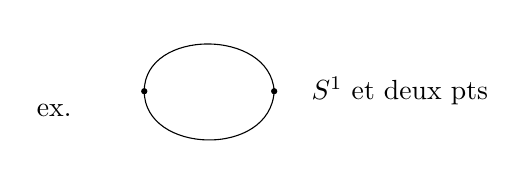
\begin{tikzpicture}[x=1cm,y=1cm]
\draw (0,0) .. controls (0,.8) and (1.6,.8) .. (1.65,0)
.. controls (1.6,-.85) and (0,-.8) .. (0,0);
\fill (0,0) circle(.04); \fill (1.65,0) circle(.04);
\node[left] at (-.8,-.25) {ex.};
\node[right] at (2,0) {$S^1$ et deux pts};
\end{tikzpicture}}}

\deleted{Li a) $C$ fermée, et $C\in\{A,B\}$ ou $C\subset U$
\inserted{$X\setminus(A\cup B)$}}

\deleted{\unsure{b)}
($C$ est l'une des extrémités, ou n'en rencontre aucune)}

Li a) $\exists$ décomposition de $X\setminus C$ en somme \inserted{\unsure{top.}} de deux sous-espaces
\[
\unsure{\deleted{U}\inserted{X}|\deleted{X}\inserted{U}}_{A,C},\quad \unsure{\deleted{U}\inserted{X}|\deleted{X}\inserted{U}}_{B,C}
\]
\[
A\subset\unsure{\deleted{U}\inserted{X}|\deleted{X}\inserted{U}}_{A,C}
\qquad
B\subset\unsure{\deleted{U}\inserted{X}|\deleted{X}\inserted{U}}_{B,C}
\]
et
\[
\unsure{\deleted{U}\inserted{X}|\deleted{X}\inserted{U}}_{A,C}/A
\quad\text{et}\quad
\unsure{\deleted{U}\inserted{X}|\deleted{X}\inserted{U}}_{B,C}/B
\]
connexes
[et ceci détermine $X_{A,C}$, $X_{B,C}$ de façon unique,
comme images inverses des comp. conn. de
$\underset{\inserted{\begin{array}{c}\unsure{\Vert|\text{''}}\\{}_A\backslash X/B\end{array}}}{X'}\setminus C$
qui contient

\margin{i.e. $X'\setminus C$ a deux comp. connexes, dont l'une contient $a$, l'autre contient $b$}

\margin{\uline{NB} \unsure{Quand} $A,B$ connexes,
$U_{A,C}$, $U_{B,C}$ \deleted{\unsure{sont}} sont connexes
donc \unsure{les c.c.} de $X\setminus C$}

\rotatebox{90}{\reflectbox{\unsure{EXTRA STRONG}}}
\rotatebox{90}{\reflectbox{\unsure{EXTRA STRONG}}}
\mspage{4}
